% All options passed to `tui-algo-seminar` get passed through to lipics-v2021.
% Read its documentation for a reference:
% https://submission.dagstuhl.de/series/details/5#author
\documentclass[a4paper,german]{tui-algo-seminar}

% (Un-)comment these at will:
\usepackage{graphicx}
\usepackage{algorithm2e}  % pseudocode listings
\usepackage{booktabs}  % better-looking tables
\usepackage{tikz}  % draw figures

\seminar{Hauptseminar Informatik (Bachelor)}
%\seminar{Hauptseminar Informatik (Master)}
%\seminar{Proseminar Informatik (Bachelor)}

\semester{Wintersemester 2022/23}
\title{Your Title}
\author{Jane Doe}

% Uncomment this to remove line numbers.
% Line numbers must be included in any preliminary version.
% \nolinenumbers  % this command is defined by package `lineno`


\begin{document}

\maketitle

\begin{abstract}
Hier schreiben Sie einen Abstract für Ihre Ausarbeitung.
\end{abstract}


\section{Einleitung}

\subsection{Die \texttt{tui-algo-seminar}-Klasse}

\begin{itemize}
	\item Mit den Argumenten \texttt{german} oder \texttt{english} können Sie die Titel der Theorem-environments entsprechend umbenennen, z.B. \enquote{Beweis} oder \enquote{Proof}.
  \item Benutzen Sie den \texttt{\textbackslash enquote\{\}}-Befehl vom Paket \texttt{csquotes} für Anführungszeichen.
  \item Sie können außerdem das \texttt{booktabs}-Paket verwenden,
    welches Ihnen das Erstellen schöner Tabellen erleichtert.
    In Tabelle~\ref{tab:interessante-tabelle} sehen Sie ein Beispiel dafür.
  \item Im Appendix~\ref{sec:itemStyles} und~\ref{sec:theorem-environments} sehen Sie Beispiele für Aufzählungs- und Theorem-Umgebungen.
\end{itemize}

\section{Weitere nützliche Hinweise}
\label{sec:weitere_nutzliche_hinweise}

\begin{enumerate}
  \item Tutorials für \LaTeX{} finden Sie bspw. auf Wikibooks unter der folgenden Adresse: \\ \url{https://de.wikibooks.org/wiki/LaTeX-Kompendium}.
  \item Verwalten Sie die \LaTeX-Dateien für Ihre Ausarbeitung in overleaf oder in einem \texttt{git}-Repository und legen Sie regelmäßig Backups an.
  \item Wenn Ihre Ausarbeitung zu lang wird, teilen Sie sie mit \texttt{\textbackslash include} in mehrere Dateien auf.
\end{enumerate}


\section{Ein anderer Abschnitt}

Mit dem \texttt{\textbackslash section\{\}}-command können Sie eine Überschrift definieren.

\subsection{Abbildungen, Tabellen und Pseudocode}

\begin{figure}[ht]
	\centering
	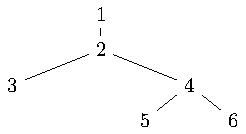
\includegraphics[scale = 0.7]{figures/figure-1.pdf}
	\caption{Dies ist Abbildung, die als PDF eingebunden wurde.}
	\label{fig:picture}
\end{figure}

\begin{figure}
	\centering
	\begin{tikzpicture}
		\tikzstyle{level 1}=[sibling distance=60mm,level distance=.6cm]
		\tikzstyle{level 2}=[sibling distance=30mm,level distance=.6cm]
		\tikzstyle{level 3}=[sibling distance=15mm,level distance=.6cm]
		\tikzstyle{level 4}=[sibling distance=10mm,level distance=.6cm]

		\node at (0,0) {7}
		child{ node{2}
			child{ node{1} }
			child{ node{4}
				child{ node{3} }
				child{ node{6} }
			}
		}
		child{ node{14}
			child{ node{12}
				child{ node{9}
					child{ node{8} }
					child{ node{11} }
				}
				child{ node{13} }
			}
			child{ node{16}
				child{ node{15} }
				child[missing]{}
			}
		};
	\end{tikzpicture}
	\caption{Dies ist eine mit TikZ generierte Abbildung eines Binärbaums.}
	\label{fig:binary-tree}
\end{figure}

\begin{table}[ht]
\centering
\caption{Diese Beispiel-Tabelle ist aus der \texttt{booktabs}-Dokumentation entnommen.}
\begin{tabular}{llr}
	\toprule
	\multicolumn{2}{c}{Artikel} \\
	\cmidrule(r){1-2}
	Tier & Beschreibung & Preis (€) \\
	\midrule
	Mücke & pro Gramm & 13.65 \\
				& pro Stück & 0.01 \\
	Gnu   & ausgestopft & 92.50 \\
	Emu   & ausgestopft & 33.33 \\
	Gürteltier & gefroren & 8.99 \\
	\bottomrule
\end{tabular}
\label{tab:interessante-tabelle}
\end{table}

\begin{algorithm}[ht]
  \caption{Ein Greedy-Algorithmus, gesetzt mit \texttt{algorithm2e}}
  \KwIn{Menge $\mathcal{C}$ aller Kreise in $G=(V,E)$.}
  \KwOut{Kreisbasis minimalen Gewichts von $G$.}
  Sortiere $\mathcal{C}$ aufsteigend nach Gewicht zu $C_1,\ldots,C_k$\;
  $\mathcal{B}^\star$ $\leftarrow$ $\emptyset$\; %
    \For{$i = 1$ \KwTo $k$}{ %
      \If{$\mathcal{B}^\star \cup \{C_i\}$ linear unabhängig}{ %
        $B^\star$ $\leftarrow$ $B^\star \cup \{C_i\}$\;
      }
  }
\end{algorithm}

\subsection{Beispiele für Referenzen}
\label{sub:beispiele_fur_referenzen}

Das erste Beispiel \cite{DBLP:journals/cacm/Knuth74}, das zweite Beispiel
\cite{DBLP:journals/cacm/Dijkstra68a} und  das dritte Beispiel \cite{DBLP:books/mk/GrayR93, DBLP:conf/focs/HopcroftPV75}
für eine Referenz.

\nocite{DBLP:conf/focs/FOCS16}


\bibliography{references}


\appendix

\section{Styles of lists, enumerations, and descriptions}
\label{sec:itemStyles}

List of different predefined enumeration styles:

\begin{itemize}
\item \verb|\begin{itemize}...\end{itemize}|
\item \dots
\item \dots
%\item \dots
\end{itemize}

\begin{enumerate}
\item \verb|\begin{enumerate}...\end{enumerate}|
\item \dots
\item \dots
%\item \dots
\end{enumerate}

\begin{alphaenumerate}
\item \verb|\begin{alphaenumerate}...\end{alphaenumerate}|
\item \dots
\item \dots
%\item \dots
\end{alphaenumerate}

\begin{romanenumerate}
\item \verb|\begin{romanenumerate}...\end{romanenumerate}|
\item \dots
\item \dots
%\item \dots
\end{romanenumerate}

\begin{bracketenumerate}
\item \verb|\begin{bracketenumerate}...\end{bracketenumerate}|
\item \dots
\item \dots
%\item \dots
\end{bracketenumerate}

\begin{description}
\item[Description 1] \verb|\begin{description} \item[Description 1]  ...\end{description}|
\item[Description 2] Fusce eu leo nisi. Cras eget orci neque, eleifend dapibus felis. Duis et leo dui. Nam vulputate, velit et laoreet porttitor, quam arcu facilisis dui, sed malesuada risus massa sit amet neque.
\item[Description 3]  \dots
%\item \dots
\end{description}

% Pass cleveref / autoref to tui-algo-seminar
% if you want to use the cleveref or autoref packages.
% \cref{testenv-proposition} and \autoref{testenv-proposition} ...

\section{Theorem-like environments}
\label{sec:theorem-environments}

List of different predefined enumeration styles:

\begin{theorem}\label{testenv-theorem}
Fusce eu leo nisi. Cras eget orci neque, eleifend dapibus felis. Duis et leo dui. Nam vulputate, velit et laoreet porttitor, quam arcu facilisis dui, sed malesuada risus massa sit amet neque.
\end{theorem}

\begin{lemma}\label{testenv-lemma}
Fusce eu leo nisi. Cras eget orci neque, eleifend dapibus felis. Duis et leo dui. Nam vulputate, velit et laoreet porttitor, quam arcu facilisis dui, sed malesuada risus massa sit amet neque.
\end{lemma}

\begin{corollary}\label{testenv-corollary}
Fusce eu leo nisi. Cras eget orci neque, eleifend dapibus felis. Duis et leo dui. Nam vulputate, velit et laoreet porttitor, quam arcu facilisis dui, sed malesuada risus massa sit amet neque.
\end{corollary}

\begin{proposition}\label{testenv-proposition}
Fusce eu leo nisi. Cras eget orci neque, eleifend dapibus felis. Duis et leo dui. Nam vulputate, velit et laoreet porttitor, quam arcu facilisis dui, sed malesuada risus massa sit amet neque.
\end{proposition}

\begin{conjecture}\label{testenv-conjecture}
Fusce eu leo nisi. Cras eget orci neque, eleifend dapibus felis. Duis et leo dui. Nam vulputate, velit et laoreet porttitor, quam arcu facilisis dui, sed malesuada risus massa sit amet neque.
\end{conjecture}

\begin{observation}\label{testenv-observation}
Fusce eu leo nisi. Cras eget orci neque, eleifend dapibus felis. Duis et leo dui. Nam vulputate, velit et laoreet porttitor, quam arcu facilisis dui, sed malesuada risus massa sit amet neque.
\end{observation}

\begin{exercise}\label{testenv-exercise}
Fusce eu leo nisi. Cras eget orci neque, eleifend dapibus felis. Duis et leo dui. Nam vulputate, velit et laoreet porttitor, quam arcu facilisis dui, sed malesuada risus massa sit amet neque.
\end{exercise}

\begin{definition}\label{testenv-definition}
Fusce eu leo nisi. Cras eget orci neque, eleifend dapibus felis. Duis et leo dui. Nam vulputate, velit et laoreet porttitor, quam arcu facilisis dui, sed malesuada risus massa sit amet neque.
\end{definition}

\begin{example}\label{testenv-example}
Fusce eu leo nisi. Cras eget orci neque, eleifend dapibus felis. Duis et leo dui. Nam vulputate, velit et laoreet porttitor, quam arcu facilisis dui, sed malesuada risus massa sit amet neque.
\end{example}

\begin{note}\label{testenv-note}
Fusce eu leo nisi. Cras eget orci neque, eleifend dapibus felis. Duis et leo dui. Nam vulputate, velit et laoreet porttitor, quam arcu facilisis dui, sed malesuada risus massa sit amet neque.
\end{note}

\begin{note*}
Fusce eu leo nisi. Cras eget orci neque, eleifend dapibus felis. Duis et leo dui. Nam vulputate, velit et laoreet porttitor, quam arcu facilisis dui, sed malesuada risus massa sit amet neque.
\end{note*}

\begin{remark}\label{testenv-remark}
Fusce eu leo nisi. Cras eget orci neque, eleifend dapibus felis. Duis et leo dui. Nam vulputate, velit et laoreet porttitor, quam arcu facilisis dui, sed malesuada risus massa sit amet neque.
\end{remark}

\begin{remark*}
Fusce eu leo nisi. Cras eget orci neque, eleifend dapibus felis. Duis et leo dui. Nam vulputate, velit et laoreet porttitor, quam arcu facilisis dui, sed malesuada risus massa sit amet neque.
\end{remark*}

\begin{claim}\label{testenv-claim}
Fusce eu leo nisi. Cras eget orci neque, eleifend dapibus felis. Duis et leo dui. Nam vulputate, velit et laoreet porttitor, quam arcu facilisis dui, sed malesuada risus massa sit amet neque.
\end{claim}

\begin{claim*}\label{testenv-claim2}
Fusce eu leo nisi. Cras eget orci neque, eleifend dapibus felis. Duis et leo dui. Nam vulputate, velit et laoreet porttitor, quam arcu facilisis dui, sed malesuada risus massa sit amet neque.
\end{claim*}

\begin{proof}
Fusce eu leo nisi. Cras eget orci neque, eleifend dapibus felis. Duis et leo dui. Nam vulputate, velit et laoreet porttitor, quam arcu facilisis dui, sed malesuada risus massa sit amet neque.
\end{proof}

\begin{claimproof}
Fusce eu leo nisi. Cras eget orci neque, eleifend dapibus felis. Duis et leo dui. Nam vulputate, velit et laoreet porttitor, quam arcu facilisis dui, sed malesuada risus massa sit amet neque.
\end{claimproof}

\end{document}
